\documentclass[border=3pt]{standalone}
\usepackage{xcolor}
\usepackage{tikz}
\usetikzlibrary{arrows.meta,decorations.pathreplacing}

\definecolor{fieldblue}{HTML}{0369A1}
\definecolor{fieldorange}{HTML}{EA580C}
\definecolor{fieldink}{HTML}{334155}

\begin{document}
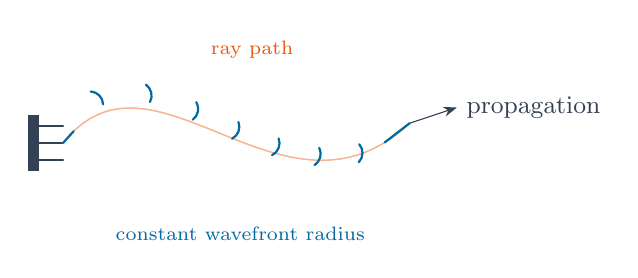
\begin{tikzpicture}[>=Stealth,line cap=round]
  \fill[fieldink] (-2.5,-.35) rectangle (-2.35,.35);
  \draw[fieldink,line width=.8pt] (-2.35,0) -- (-2.05,0);
  \draw[fieldink,line width=.8pt] (-2.35,.22) -- (-2.05,.22);
  \draw[fieldink,line width=.8pt] (-2.35,-.22) -- (-2.05,-.22);

  \draw[fieldorange!45,line width=.55pt]
    (-2.05,0) .. controls (-.9,1.45) and (.75,-1.25) .. (2.35,.25);
  \draw[fieldblue,line width=.8pt,decorate,
    decoration={waves,segment length=5.5mm,radius=1.7mm,angle=42,
      pre length=2mm,post length=4mm,raise=1mm}]
    (-2.05,0) .. controls (-.9,1.45) and (.75,-1.25) .. (2.35,.25);

  \draw[-Stealth,fieldink] (2.35,.25) -- (2.95,.45)
    node[right,font=\small] {propagation};
  \node[fieldorange,anchor=south,font=\scriptsize] at (.35,.95)
    {ray path};
  \node[fieldblue,anchor=north,font=\scriptsize] at (.2,-.95)
    {constant wavefront radius};
\end{tikzpicture}
\end{document}
